This section describes an alternative to the method presented in the previous section. Instead of calculating the proportion of true positives in the population, the samples of the Govdocs1 dataset that are labeled ``structured'' are used as input to train a second model, that will be used to validate the first model.

% \levelC{Dataset}
The model training was divided into two passes, depicted in Figure \ref{fig:randommeasure}. Each pass trains a different model for each file type. In the first pass, the dataset creation of a given file type follows the same procedure mentioned in the previous section.

\noindent
\begin{figure*}[htb!]
\centering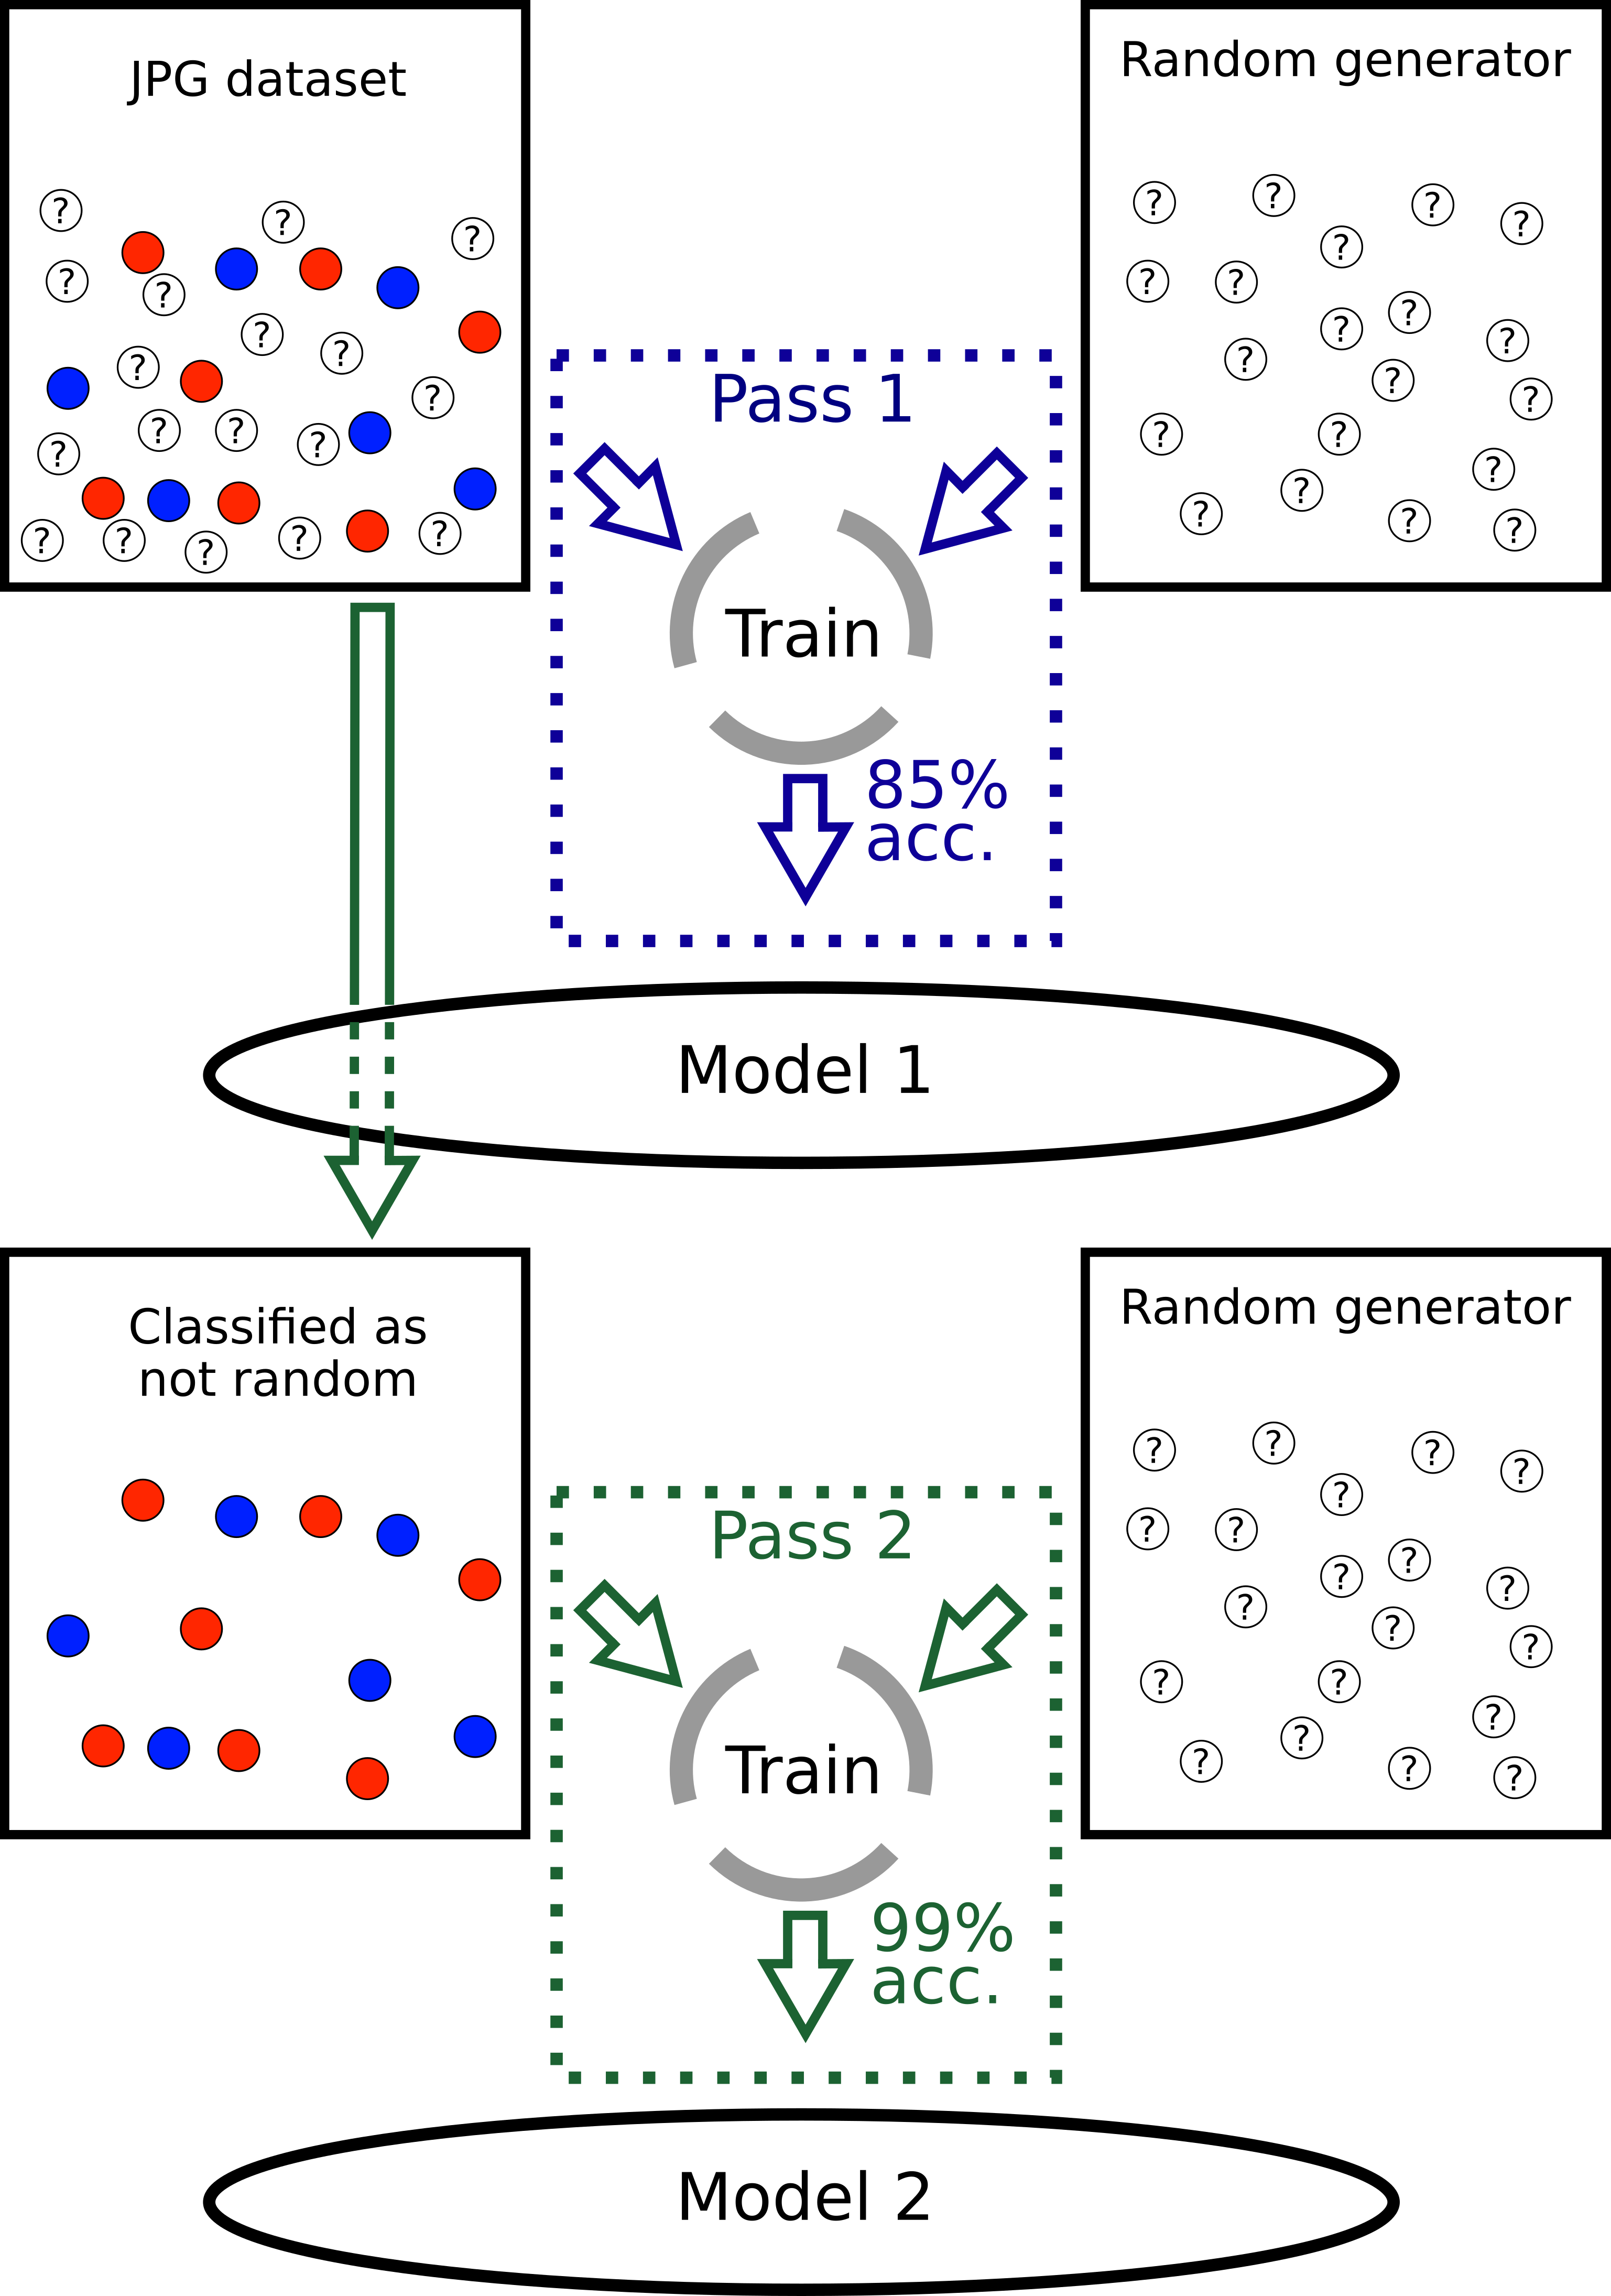
\includegraphics[width=0.5\textwidth]{content/random_measure.png}
\caption{\label{fig:randommeasure}Example of the random measure for the JPG file type. In pass 1, a model is trained to classify the data as ``random'' or ``structured'', achieving 87\% accuracy. In pass 2, another model is trained to do the same task, but the JPG blocks used are those classified as ``structured'' by model 1. As model 2 achieves an accuracy of 99\%, it validates that almost all the blocks classified as ``structured'' by model 1 are indeed not random. Then model 1 can be used to make an upper boundary estimate of the randomness of the dataset.}%
\end{figure*}
\todo[inline]{update figure and label to reflect results}

When the model training finishes the first pass, if the validation accuracy is above a predefined threshold (98\% in this study) for a given file type, no further passes are required by that file type, as the model already can distinguish between ``random'' and ``structured'' classes for that particular file type. This will only happen on file types that have almost no random-like structures.

In the second pass, the file type dataset is filtered and only those fragments classified as ``structured'' in the first pass are used in the second pass. The random generator does not require similar filtering. If in the second pass the accuracy is above the predefined threshold, it means that the first pass successfully selected samples that have almost no random-like structures. In that case, the model of the first pass can then be used in the original dataset, giving a count of how many fragments are correctly identified as ``structured''. In this particular case, the model of the first pass can be used to filter the dataset, hence the method name, as it can split the data with almost no false positives.

If the second pass accuracy is below the threshold, the equations used in the previous section can be used on the results of the second pass, to avoid further passes.

